\chapter{Background and Related Work}
\label{chp2}


Every day, new technologies are brought to practice from labs, provide convenience to daily life, and promote advances in human culture. Among these technologies, the emerging of text searching engines like google is a great milestone. Retrieving images~\citep{bisearch} or other multi-media data  in a way similar to retrieving text is even more attractive, especially for the popularity of smart phones nowadays. There are still technical obstacles for this beautiful outlook. Deciding semantic labels for images is one, and detection of target objects from images is another. The efforts in this thesis try to contribute to detecting target objects from images or image sequences.

This chapter first discusses possible advantages in human beings' visual perception against machines, and how these advantages will activate new machine vision methods in Section \ref{ch2vh}. Then abstractions in artificial intelligence which are closely related to machine vision are reviewed in Section \ref{ch2ai}. This chapter also reviews basics and advances in visual object detection in Section \ref{ch2p3} and \ref{ch2p4}. Finally this chapter summarizes by giving why the efforts of the thesis are important in Section \ref{ch2p5}.

\section{Vision in Humans and Computers}
\label{ch2vh}
The computational power of humans is not any more competitive to computers, especially nowadays, when computational resources can be conveniently accessed from the cloud.
Still when talking about the performance of visual recognition and detection under general situations, humans are still champions. In computer vision area, besides bar scanners and optical character recognition, few detection methods are employed in real-world applications, except that face detection methods are employed in ordinary cameras.

So what stops the object detection methods of computers from performing as good as those of humans?

\begin{table}[h]
\centering
\begin{tabular}{lcc}
     \hline
     \hline
                               &	Computers & Humans \\
    Quality of sensors         &	* &   \\
    Computational capability      &	* &	  \\
    Representative model       &	  & * \\
    Decision making procedure         &      & *	  \\
    Information fusion mechanisms & & *           \\
    Training quality           &      & *	   \\
   \hline
\end{tabular}
\caption[Comparisons in visual capabilities between computers and humans]{Comparisons of visual capabilities between computers and humans.}\label{c2tb:tb1}
\end{table}

When compared with humans, computers will win at almost every aspect of hardware, as shown in Table \ref{c2tb:tb1}. Besides visual sensors, new sensors are continuously developed for computers, and computers have so many choices for sensors of very high quality. What is worth mentioning is how Microsoft's Kinect advances pose recognition~\citep{knct}. Especially, for computational ability,~\citep{bpw} believes human brains have a raw computational power between $10^{13}$ and $10^{16}$ operations per second, and modern computers are much more powerful.

 As for representative model, there is no obvious evidence which proves humans are doing better than computers. While representative models of humans have long been working as inspirations and benchmarks for those of computers~\citep{rbm}. However the author believes that humans shall perform better than computers in the aspects of software, which then explains why humans perform better in multiple visual tasks. And only when the vision researchers also believe so, do they develop  so many new detection methods. And the  dividing of functionalities  are generally based on computers, while in humans, two or more of them might work together.

Human babies are taken good care of, and trained to perform very simple visual tasks for months with large amounts of examples, which makes the training quality very solid. The performance of new born babies also leads to considerations about what percentage the visual abilities in human are decided by their genes. If the training procedure has taken as long as millions of years, are there possibilities for computers to win in future?

The success of auditory speech recognition and its successful deployment in industry~\citep{siri} encourage vision researchers. Also new sensors advance recognition performance, such as Kinect, which can hopefully fill the gap of representative models' quality between computers and humans. Object recognition methods based on 2D images with 3D model~\citep{r3d} also makes it possible for computers to share similar representative models with humans.  Computational power can be used to make up with the short slab of training. For example, training one model for relative small amount of time with thousands of computers~\citep{dnnnn} is feasible with parallel training. The recent deep learning~\citep{dlearn} methods try to fusion representative model with decision making procedure to act more like what humans might do. These new achievements are expected to fill up the gap between humans and computers in aspects of representative model, decision making procedure, and training quality.



While the methods proposed in this thesis explore the information which can be further made use of, i.e., fusion of temporal and visual information, and fusion of the visual and spatial information of different parts of the same object. The efforts here shall belong to decision making procedure, and information fusion mechanism. Especially, in Chapter \ref{chp4}, a perceptual mechanism in human are combined into a voting system, and this results in a detection method with promising detection performance.

\section{Artificial Intelligence}
\label{ch2ai}
AI (Artificial Intelligence) includes a very wide range of topics, of which, computer vision is comparably difficult.

The author of this thesis is positive about that fact that computers can outperform humans in visual tasks for the reasons in the previous section. Then if we move towards the correct direction, one step forward will lead to one step nearer to this goal, and vice versa.

Needless to say, the core of Artificial Intelligence is operations at high abstraction levels. When talking about the abstraction level of computer vision, the area of text mining can be used as a benchmark, though such comparisons will not be fair. Texts themselves are at a higher abstraction level than images. And the achievements in text understanding will remind the researchers of computer vision about the unsatisfactory results of turning images to semantic labels.

Together with lots of researchers in computer vision, the author of this thesis believes achievements in abstraction of a higher level will help with the results in low abstraction levels. Something which can only be proven by time is that if the computer vision problems of low abstraction levels draw too much attention, it will not benefit the area.


Taking the problems of multi-class detection as example, routines of different types will be discussed. One routine is to explore detection of object from multiple classes at the same time. This kind of routine has been followed a lot by researchers, especially those encouraged by some recent competitions on visual tasks, e.g., VOC2012~\citep{voc}. Significant amount of engineering efforts are needed to win this kind of competitions. Another routine is that
development of mechanisms of high abstraction level for single-class detection and mechanisms to separate objects from different classes. The problem with the first routine is that, methods will be so limited to the training dataset, and mechanisms at higher levels which are very valuable are not easy to explore.

Actually, perceptual mechanisms in humans are consistent with the above arguments. Recall how humans are capable of detecting previously unseen objects, while they acquire knowledge of target objects through verbal descriptions.

The methods proposed in this thesis explore the detection procedure at a high abstraction level.

\section{Basics of Detection Methods}
\label{ch2p3}
In the previous section, the possible reason how humans perform better in detection is discussed. The main limitations of computers are of software. Based on this, researchers present new detection methods or new methods for supporting detection, which includes: 1) new image features or new representative models, 2) new decision making procedures, or 3) better searching techniques in solution space.
\subsection{Image Features}
Image features are very important. Simple image features include features in the form of keypoints, image patches, edges,  silhouette, shape~\citep{scontext}, or textures. There are also frameworks for combining multiple different image features or information from multiple channels~\citep{regionc,bgf,lbp,lss}, and these belong to image features at middle level~\citep{midf}. At an even higher level, image features can be  organized in patterns. For example, modeling human body as a stick model~\citep{stickb}.

The invariance under illumination, scale, and rotation are basic requirements for image features, while some keypoint features~\citep{ij2,o12,o14,o15,o2} fulfill these requirements. Image features which encode global positional information perform well in human detection, i.e., Histograms of Oriented
Gradients~\citep{ij4}. Differentials at different orders can also be used as descriptive features~\citep{regionc}.



\subsection{Decision Making Procedure}
Generally, robustness and computational efficiency are the two main pursues in proposing image features. Based on image features, how decisions are made are also of great importance. Dimension reduction methods like principal component analysis, and feature selection methods can be considered as a glue layer between representative models and decision making procedure, which enhance both robustness and processing efficiency.

The are mainly two main categories of methods for decision making: discriminative methods, and generative methods.
Support vector machine, and boosting methods belong to discriminative methods. Gaussion processes~\citep{gprocess}, Dirichlet models~\citep{lda,dp,hdp}, and Bayesian graphical models~\citep{bgm} usually belong to generative methods. The differences between discriminative and generative models lay in how they use training examples to estimate parameters of the model, and how the model is used to make decisions.

One very promising method for decision making is deep learning~\citep{dlearn}. This can be considered as a special form of neural network. One of its very attractive property is that it can take raw data as input and output decision results, like, object label. It deals with extraction of image feature, feature selection, and decision based on features in a unified model under the same framework. Also it can share knowledge from other domain like~\citep{tlsurvey}.

The core of machine learning methods is still the model. Training data are used to estimate  parameters of the model, and the model is then used to make decisions on the testing data. The model of deep learning is a multi-layer network. The later one layer is, usually it has less nodes, and the information it deals with is more abstract.

The earlier layers of deep-architecture networks act as feature extraction module. The first layer defines rules of how to make abstraction on the raw data. And these layers can be trained using  data from other domains. This is why deep learning methods can make use not only domain-specific information. Another aspect which separates deep learning methods from traditional neural networks lies in the training procedure. Traditional neural networks are trained as a whole, which means the inferring for lots of parameters at the same time, and good training quality  requires extremely large amount of data. The training procedure for deep learning methods is layer-wised. There is a merit for evaluate the training quality for each layer. And after one layer is trained, the output can be used to train the next layer. This means that, each time only a few parameters need to be estimated, which is more robust and efficient, and avoid the requirement for very large amount of data. When the number of layers increase, the abstraction level of the original data enhance, and decisions are easier.


\subsection{Solution Space Exploring}
Besides proposing representative models and decision making procedures, there are lots of work~\citep{408,spm,ciod} focusing on how the solution space from the decision making procedure can be explored. The methods following the sliding-window schema need to check each differently scaled sub-image of a target image, and answer whether this sub-image contains an object of interest. While the number of all sub-windows is extremely large, and even enumerating all the sub-windows is computationally infeasible.

Currently method of~\citep{ij15} and its variants~\citep{ac1} for sliding window search work very efficiently, and give best detection hypothesis in polynomial time in experiments. There are variants of~\citep{ac27} which share the same strategy for methods based on Hough transforms. These methods employ branch-and-bound mechanisms during the search for the best detection hypothesis. While map-and-reduce is popular in distributed computations, the underlining philosophy is very similar.

Take the testing process of linear support vector machine as an example. When a sub-image is described as a bag of features, each feature will contribute to a specific dimension on the final descriptive vector.
And when using this vector by support vector machine for decisions, it is simple linear add-up of the decisions of each single feature. So decision score for each image feature can be calculated. Thus the upper-bound and low-bound for all sub-images contained in a certain rectangle can be estimated, which can be used to filter out lots of rectangles definitely do not contain the best solution. This filtering out is the core for efficiency.

\section{Advances in Object Detection}
\label{ch2p4}
Three methods will be proposed in the thesis, and methods most related to each method will be further reviewed in the corresponding chapter. Here we review some recent advances in object detection.

Detection is drawing a lot of attention~\citep{ij4,ac31,ac30,ac4,ac32,ac29,ac28,ac1,ac9,ac2,ac3,ac22,lb1,ac5,ac10,ac21,ac18}, and it will continue to. While some methods are unique and very heuristic.

Instead of proposing class-specific methods,~\citep{wiao} tries to evaluate how like a sub-image contains an object of any class. In the method objects are defined by very general properties, which include having closed boundary, being different from surroundings, and sometimes being unique and salient in the image. By combining saliency detection, color contrasting, edge detection, and image segmentation methods in a Bayesian framework, they give convincing performance in general-purpose object detection.

Bag of image features~\citep{bgf} is an important advance for object detection. Before the method, potential objects are described using feature extracted from raw pixels, while the method describes objects using object components. In the work following,~\citep{ij13} added a biased sampling component for describing each object. Instead of being described by one group of features, the objects are described by several groups of features, and then decisions are made using multi-label multi-class classification.

Some pioneer methods also detect or recognize objects in 3D space. The method proposed in~\citep{r3d}, tracks keypoints of the same object, generate features which include 3D information of the object accordingly, and feed the features to decision step. And the results are very appealing.

Also excellent performance of deep learning inspires new methods to reconsider   object representations. The discover of invariants and learning of a detector from unlabeled data are explored by~\citep{dnnnn}.


Still, one of the challenging subjects in object detection is rotation-aware detection. Lots of object detection methods ignore scale and rotation changes by using of scale- and rotation-invariant image features, i.e. SIFT.
The primary  direction of the SIFT feature is used by~\citep{ac21} for locally estimating the rotation angle of object. This method heavily relies on the SIFT features.
An object is represented by a graph with features as nodes in~\citep{ac222}, and scale- and rotation-invariant object match is made by the matching of two graphs. Instead of being a general method for object detection, this method is mainly used for object matching.
Most rotation-aware methods follow~\citep{ac20}. This method firstly trains a neural network for rotation estimation. According to the rotation estimation result, the tested sub-image is rotated to a normalized angle and then fed into other classifiers for verification of object hypothesis. Still efficient methods to robustly deal with object rotation in the detection procedure are preferred.




\begin{comment}
(a) a well-de?ned closed boundary
in space; (b) a different appearance from their surroundings [23, 25]; (c) sometimes it is unique within the image
and stands out as salient
\end{comment}
\section{Chapter Conclusion}
\label{ch2p5}
There methods are proposed in the thesis. The methods contribute to decision making in object detection. These methods try to improve existing voting systems to easily employ information in multiple channels or try to accelerate the decision making procedure by employing good mechanisms.

Human beings have their limitations in computational capabilities while perform better in visual tasks. Thus machine vision methods should make use of more information in a more effective manner to perform better. This encourages the efforts in this thesis. And especially the method of Chapter \ref{chp4} learns from one mechanism of human beings.

High abstraction level in AI will be helpful for future visual detection methods. And the method in Chapter \ref{chp3} has several layers in its pipeline, and makes it unique in detect specific objects. Information from all channels are then combined in a robust voting system for better performance.

From the basics of detection methods, it is clear decision making procedure is still the most challenging part in object detection. All methods of the thesis focus on decision making.

To summarise this chapter, the methods proposed in this thesis try to contribute to object detection by proposing effective and efficient mechanisms to combining information from multiple channels in robust voting systems. These efforts are encouraged by the human beings' amazing visual capabilities, these efforts try to act at a high abstraction level, and these efforts belong to the very challenging topic of decision making in object detection, as shown in Figure \ref{ord:contri}.


\begin{figure}
\centering
{
  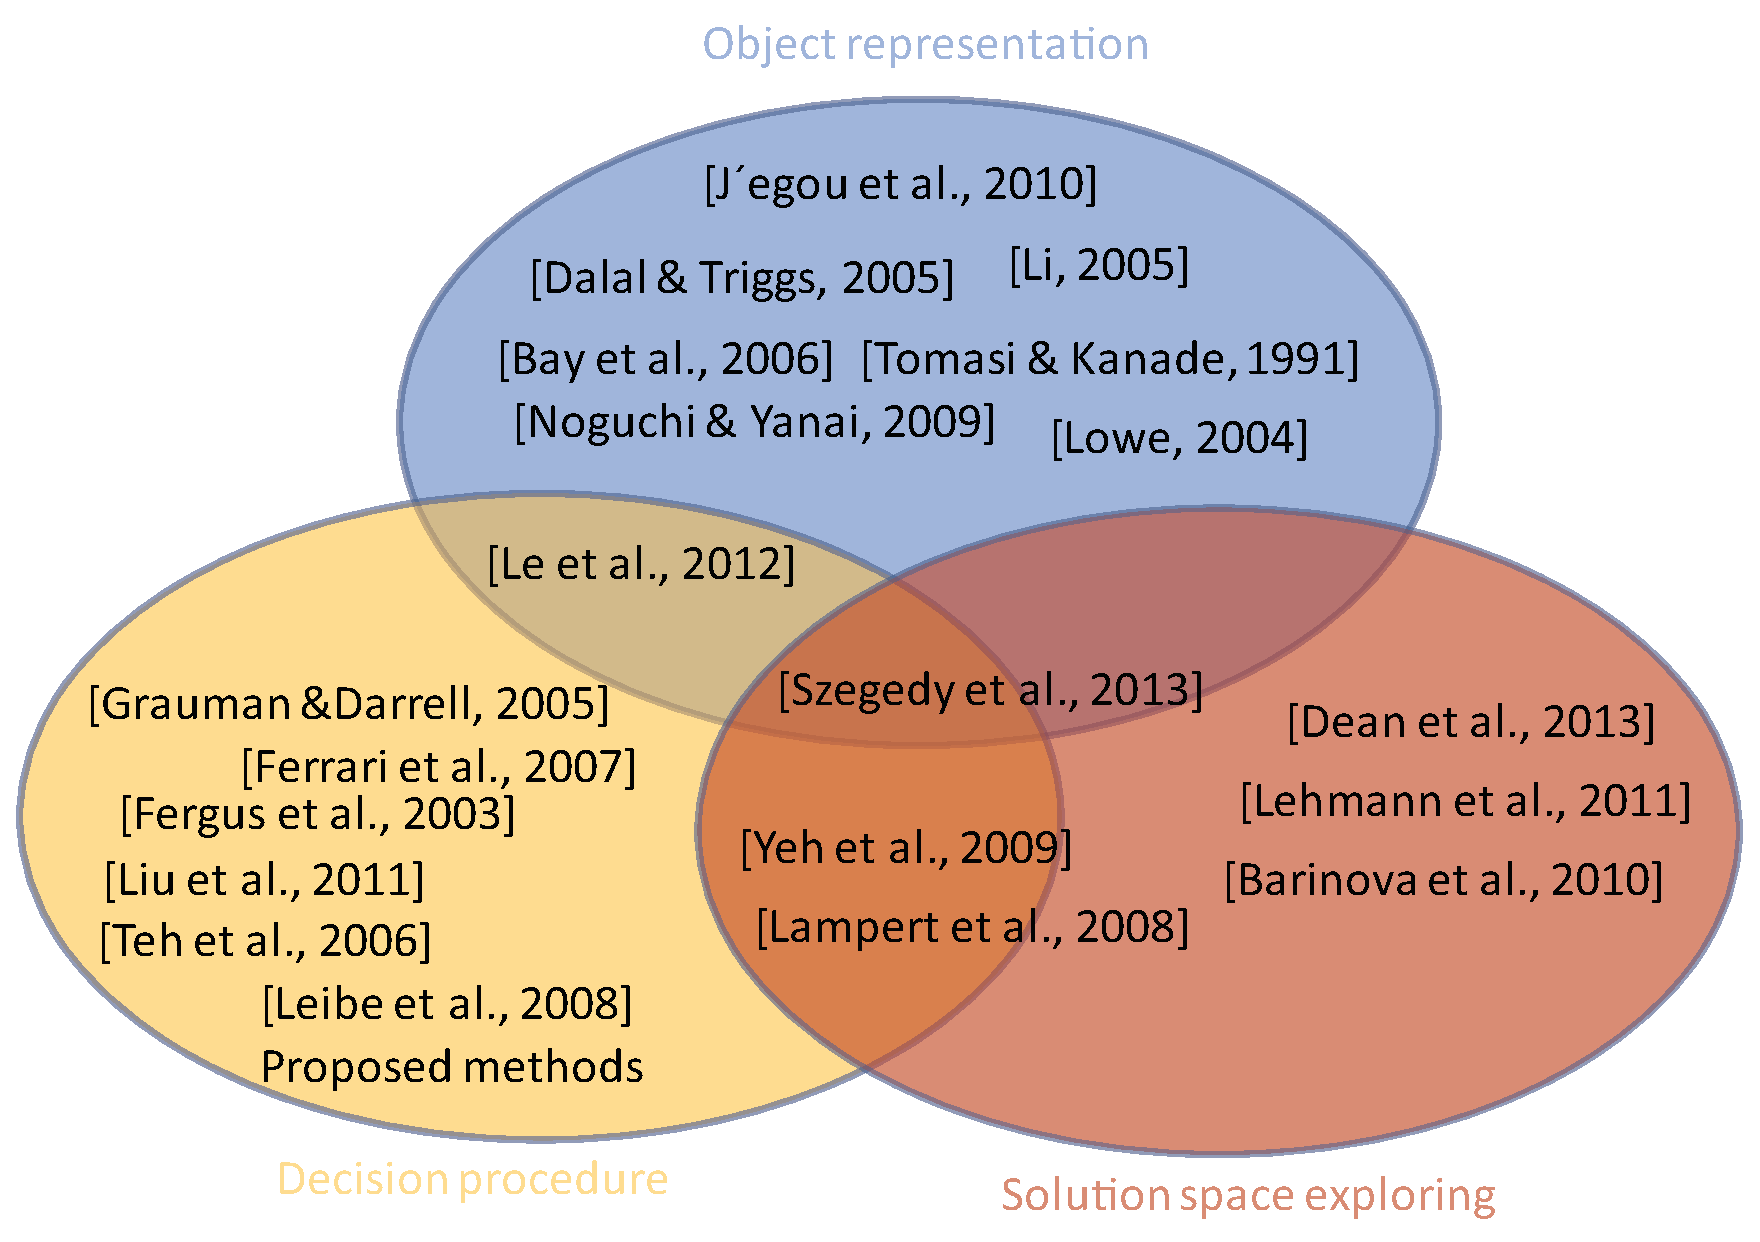
\includegraphics[width=1\textwidth]{contri.eps}
}
\caption[Categorization of contribution.]{Categorization of the contribution from the proposed methods and a few recent methods~\citep{bgf,ij4,obof,ij2,o2,mtvvv,o12,dnnnn,pmk,ac30,ac3,lbt1,hdp,lb1,ac1,ac4,408,ac27,ac9,dnnobd}.}
\label{ord:contri}
\end{figure}